\chapter{Respaldo y actualización de sitio web Wordpress}
Mantener respaldos regularmente resulta de gran importancia para asegurar la disponibilidad del sitio web del clúster para efectos de consulta y uso de sistema de Tickets recientemente implementado. De la misma forma es importante para efectos de seguridad e integridad de los equipos y bienes computacionales del CNCA mantener el software lo más actualizado posible,  sin sacrificar estabilidad. Tomando en cuenta lo anterior, se proponen lo siguiente para respaldar tanto archivos como bases de datos del sitio web, así como actualizarlo junto con sus respectivos plugins.

\section{Respaldo de archivos del sitio web}
Antes de proceder con la actualización, es de suma importancia respaldar todo lo que se tiene, pues las cosas pueden salirse de control y corromper o hasta perder de forma irreparable los datos del sitio. Algunos de los métodos sugeridos para este procedimiento se muestran a continuación.

\subsection{Cliente FTP/SFTP}
A través de la instalación y uso de un cliente FTP como Filezilla, es posible respaldar de manera remota los archivos del sitio. Iniciamos una sesión rápida con un usuario creado (los del clúster funcionan bien) al sitio cluster.cenat.ac.cr y nos conectamos al puerto 22222 para acceder al meta nodo, que es donde se encuentra el servidor (más detalles al respecto disponibles en la guía de instalación de pend), tal y como se muestra en la figura \ref{fig:wp_backup_file00}. En el panel derecho a la mitad de la pantalla se muestra el árbol de directorios del servidor. Nos dirigimos al directorio /var/www/html y procedemos a descargar el directorio wordpress, donde se incluye además los plugins instalados hasta el momento. Se recomienda, para ahorrar espacio en almacenamiento, manejar estos respaldos en archivos comprimidos, y darles un nombre distintivo que incluya la fecha del respaldo, por ejemplo wp-backup-aaaammdd.tar.gz o el compresor de preferencia.

\begin{figure}[H]
\centering
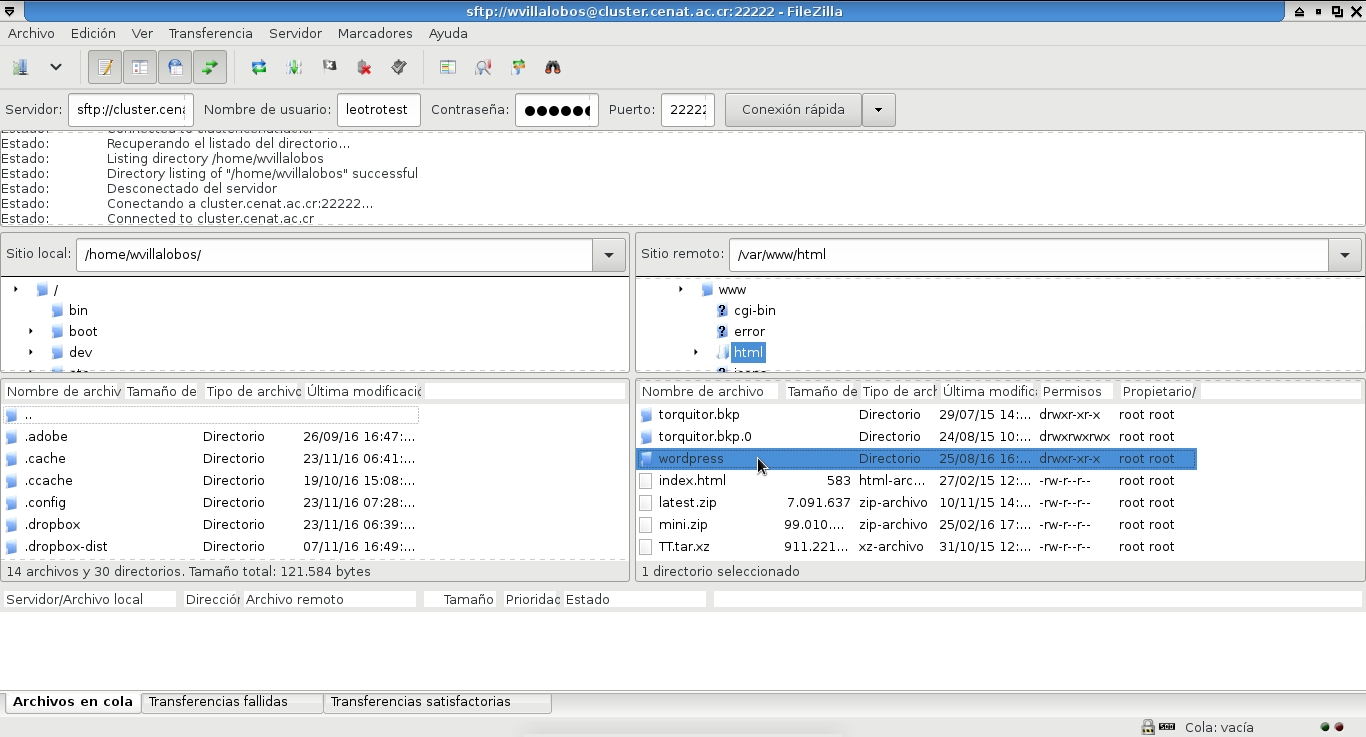
\includegraphics[width=0.5\textwidth]{wp_backup_file00}
\caption{Cliente FTP Filezilla para respaldo de archivos del sitio web.}
\label{fig:wp_backup_file00}
\end{figure}

\subsection{SFTP a través de la terminal}
El método más sencillo es quizás utilizar el cliente SFTP incluido por defecto  en la instalación del servidor SSH, el cual hemos utilizado regularmente hasta el momento. Para esto simplemente hacemos lo siguiente:

\begin{lstlisting}
sftp -p22222 leotrotest@cluster.cenat.ac.cr:/var/www/html
get -r wordpress
logout
\end{lstlisting}

Esto descargará la carpeta y sus contenidos de forma recursiva en el directorio local donde se inició la sesión remota de transferencia encriptada. De la misma forma, se recomienda manejar una nomenclatura bastante explícita y en formato comprimido. Para crear un archivo comprimido tar.gz basta con hacer lo siguiente:

\begin{lstlisting}
tar -zcvf foo.tar.gz foo
\end{lstlisting}

Para restaurar los respaldos simplemente se debe copiar el archivo comprimido de vuelta al meta nodo y descomprimirlo en el directorio correspondiente, como se muestra a continuación:

\begin{lstlisting}
scp backup.tar.gz leotrotest@cluster.cenat.ac.cr:/home/leotrotest
ssh -p22222 leotrotest@cluster.cenat.ac.cr
tar -xvzf backup.tar.gz
su
mv wordpress /var/www/html/
\end{lstlisting}

\section{Respaldo de base de datos del sitio}
Más allá de simplemente respaldar la  carpeta de archivos del sitio, es necesario respaldar la base de datos también, pues de ahí se derivan los permisos y otros detalles importantes. Para proceder con este respaldo, abrimos  un navegador web y nos dirigimos al sitio \url{cluster.cenat.ac.cr/phpmyadmin}. Nos aparecerá un cuador de diálogo de htaccess, para el cual ingresamos las credenciales de root del meta nodo. Finalmente se nos muestra una ventana como la de la figura \ref{fig:wp_backup_db00}

\begin{figure}[H]
\centering
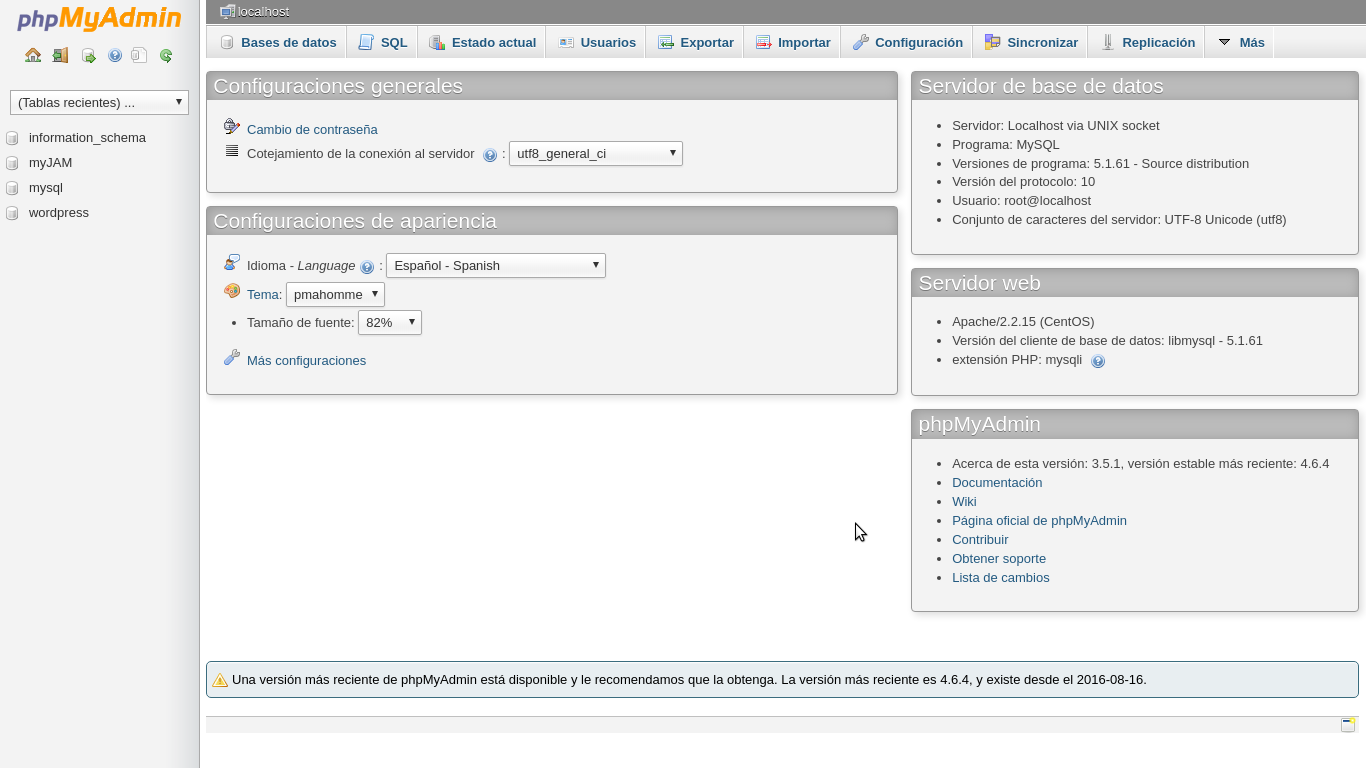
\includegraphics[width=0.5\textwidth]{wp_backup_db00}
\caption{Sitio de administración web de bases de datos phpmyadmin del meta nodo.}
\label{fig:wp_backup_db00}
\end{figure}

Seleccionamos la base  de datos correspondiente al sitio web, y nos mostrará una pantalla similar al de la figura \ref{fig:wp_backup_db01}. Acá hacemos clic en exportar
y seleccionamos la opción Personalizado y nos aseguramos de seleccionar todo, como se muestra en la figura \ref{fig:wp_backup_db02}, así como de indicar las mismas opciones, incluyendo la compresión.

\begin{figure}[H]
\centering
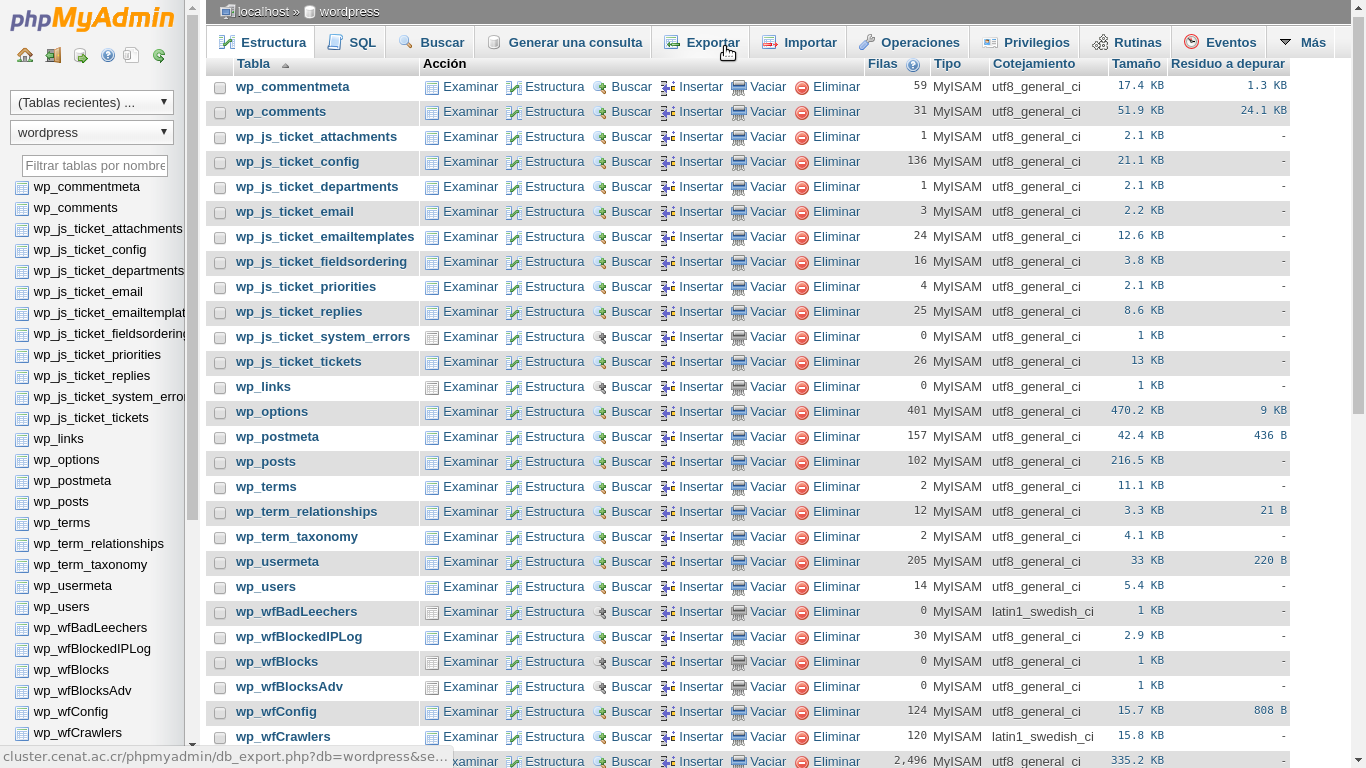
\includegraphics[width=0.5\textwidth]{wp_backup_db01}
\caption{Vista de la base de datos de wordpress mediante phpmyadmin.}
\label{fig:wp_backup_db01}
\end{figure}

\begin{figure}[H]
\centering
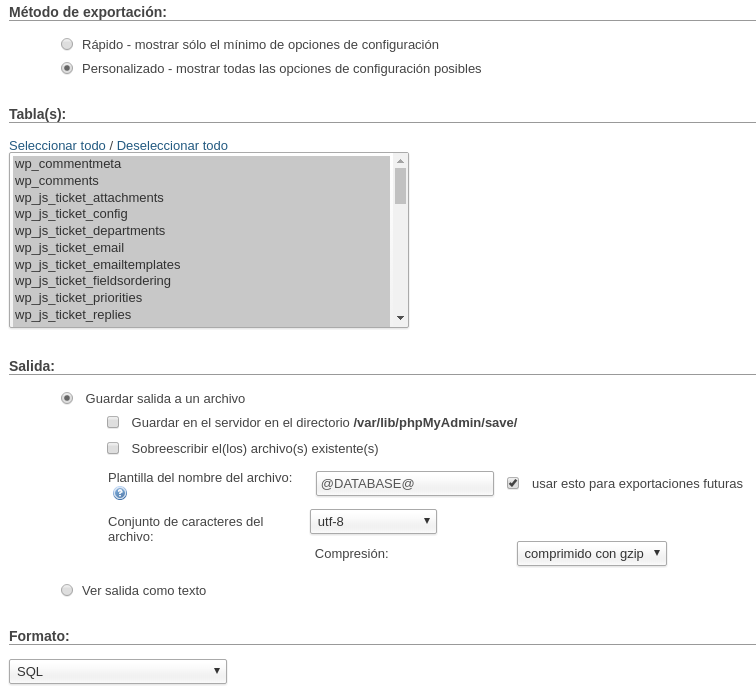
\includegraphics[width=0.5\textwidth]{wp_backup_db02}
\caption{Opciones de exportación de la base de datos.}
\label{fig:wp_backup_db02}
\end{figure}

Finalmente nos dirigimos al final y damos clic en continuar. Automáticamente iniciará la descarga del respaldo de la base de datos. Se recomiendo igualmente usar una nomenclatura explícita para este archivo.

\section{Actualización del sitio web}
Ahora procedemos a actualizar el sitio de wordpress. Primero descargamos el archivo del sitio (al momento de escribir esta guia, la versión más actualizada es la 4.6.1) \url{https://wordpress.org/download/}. Para hacerlo directamente en el meta nodo,  hacemos lo siguiente:

\begin{lstlisting}
su -
mkdir installer_wp && cd install_wp
wget https://wordpress.org/latest.tar.gz --no-check-certificate
tar -xvzf latest.tar.gz 
\end{lstlisting}

Antes de proseguir, desactivamos los plugins del sitio, como se muestra en la figura \ref{fig:wp_update00}

\begin{figure}[H]
\centering
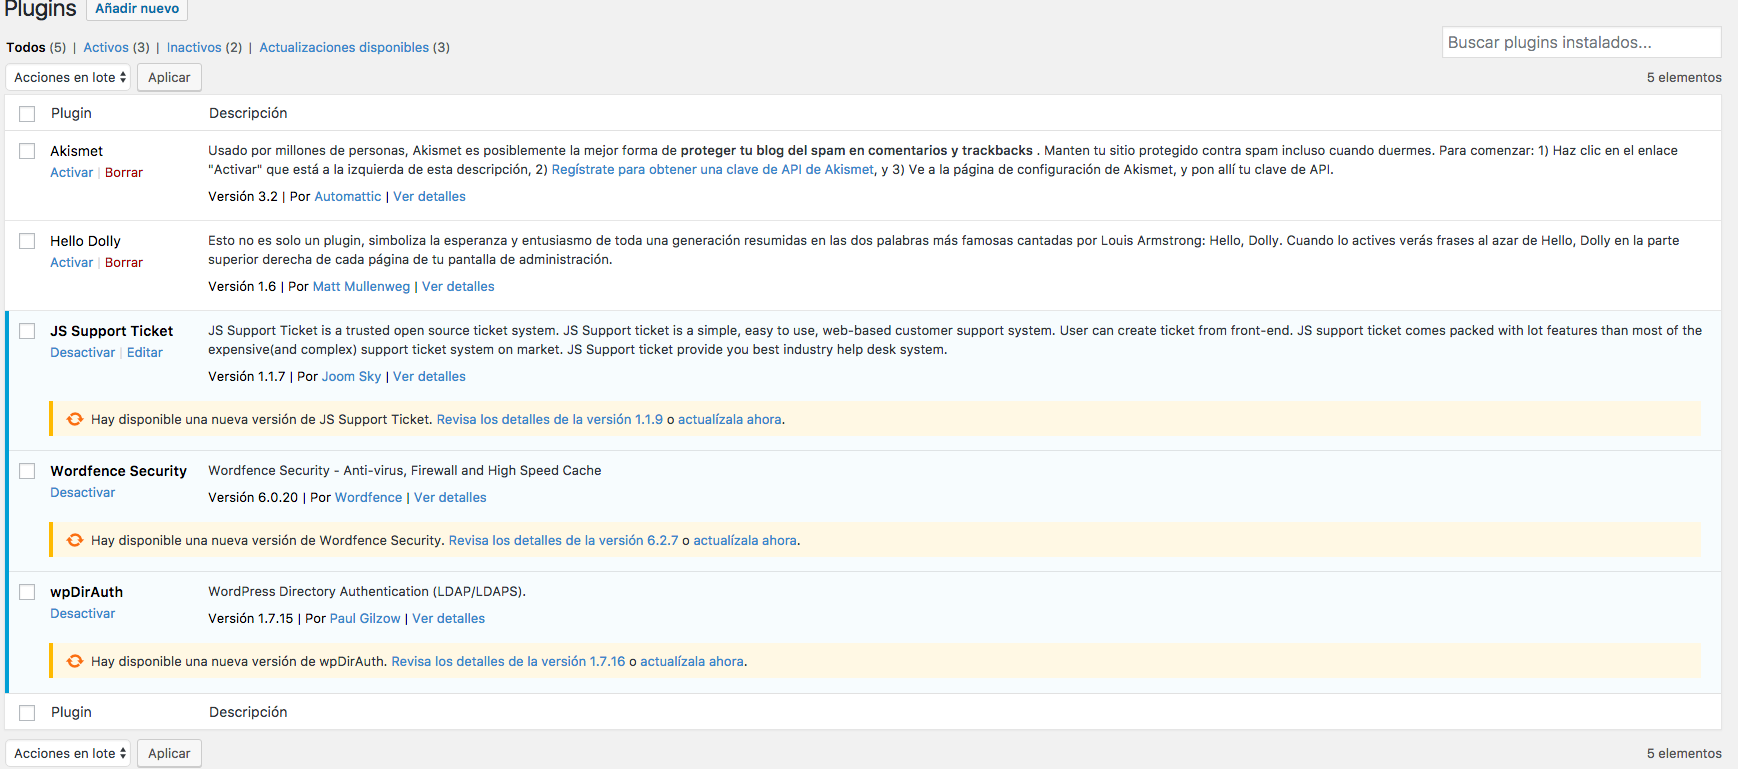
\includegraphics[width=0.5\textwidth]{wp_update00}
\caption{Desactivación de plugins para la actualización del wordpress.}
\label{fig:wp_update00}
\end{figure}

Procedemos a borrar los directorios wp-includes y wp-admin viejos y copiamos los nuevos recién descomprimidos. También nos aseguramos de copiar los contenidos de wp-content de manera que solo sobreescriba los archivos de interés, sin borrar nada de lo que tenemos adicional en este directorio.

\begin{lstlisting}
cd /root/installer_wp/wordpress
cp -r wp-admin wp-include readme.html *.php /var/www/html/wordpress
cp -r /root/installer_wp/wordpress/wp-content/* .
\end{lstlisting}

Este procedimiento puede realizarse con el cliente Filezilla de la misma forma, sin preocuparnos por sobreescribir archivos que deseamos conservar. Una vez realizado lo anterior, ingresamos al sitio \url{cluster.cenat.ac.cr/wordpress/wp-admin}. Nos mostrará una pantalla indicando que el wordpress ha sido actualizado y que se debe actualizar la base de datos, lo cual procedemos a hacer. 

\clearpage